\documentclass[11pt]{article}
\usepackage{graphicx, pdfpages, tikz, hyperref, fancyhdr,  geometry, titlesec, xcolor, csquotes, tocloft, minitoc}
\usepackage[T1]{fontenc}
\usepackage[french]{babel}

% marges du document
\geometry{
    left=3cm,
    right=3cm,
    top=2cm,
    bottom=3.5cm
}

\pagestyle{fancy}
\fancyhf{} % retirer config de page par défaut
\renewcommand{\headrulewidth}{0pt} % Supprimer la ligne d'en-tête

\fancyfoot[R]{\thepage} % numéro de page à droite
\fancyfoot[L]{{\itshape \titre}} % numéro de page à droite

\newcommand\BackgroundPic{
    \put(0,0){
        
\includegraphics[width=\paperwidth,height=\paperheight]{template/assets/template_page.pdf}
    }
}

\titleformat{\section}
  {\LARGE\bfseries\uppercase} % Mise en forme (centré, taille, gras, en majuscule)
  {\thesection}{1em}{} % Numérotation

\newcommand{\psection}[1]{\phantomsection\section*{#1}\addcontentsline{toc}{section}{#1}}

\newcommand{\aremplir}{{\LARGE \bfseries \textcolor{red}{A REMPLIR}}}

\addto\captionsfrench{
    \renewcommand{\listfigurename}{Liste des figures}%
    \renewcommand{\listtablename}{Liste des tableaux}%
}

\newenvironment{custombox}[1]{% environnement qui permet le retour à la ligne quand ça déborde
    \begin{minipage}{#1}
}{\end{minipage}} % ne pas toucher

\newcommand{\titre}{Nom du document}
\newcommand{\imagecouverture}{example-image}
\newcommand{\firstcouverture}{
    \parbox{\textwidth}{
        \textbf{Prénom NOM}\\
        Elève Ingénieur de l'INSA Toulouse\\
        Département XX\\
        Spécialité TLS-SEC\\
        Promotion XX\\
        20XX-20XX
    }
}
\newcommand{\secondcouverture}{
    \parbox{\textwidth}{
        \begin{custombox}{9cm}
            \textbf{INTITULE ICI - EXEMPLE : CONTRIBUTION A LA CONCEPTION A BAS COUT D’ANTENNES 3D}
            \vspace{1em}\\
            \textbf{Lieu du Projet de Fin d'Études ou stage}\\
            Nom de l’entreprise\\
            Adresse de l’entreprise
            \vspace{0.6em}\\
            \textbf{Tuteur du Projet (ou PFE)...}\\
            Prénom NOM du Tuteur du Projet de Fin d'Étude
            \vspace{0.6em}\\
            \textbf{Correspondant pédagogique INSA}\\
            Prénom NOM du Correspondant pédagogique INSA
            \vspace{0.6em}\\
            \textbf{PFE/Stage/Projet soutenu le 00/00/20XX}
        \end{custombox}
    }
}

% bibliographie
\usepackage{biblatex}
\addbibresource{contents/bibliography.bib}


\begin{document}
    \dosecttoc{}
\pagenumbering{Roman} % Numérotation en chiffres romains (i, ii, iii, ...)
\setcounter{page}{1}

\definecolor{couleurcarre}{HTML}{F3F0EC} 

\thispagestyle{empty} % pas de numéro de page sur cette page
\begin{tikzpicture}[remember picture, overlay]
    \node[anchor=south west, inner sep=0] at (current page.south west) {
        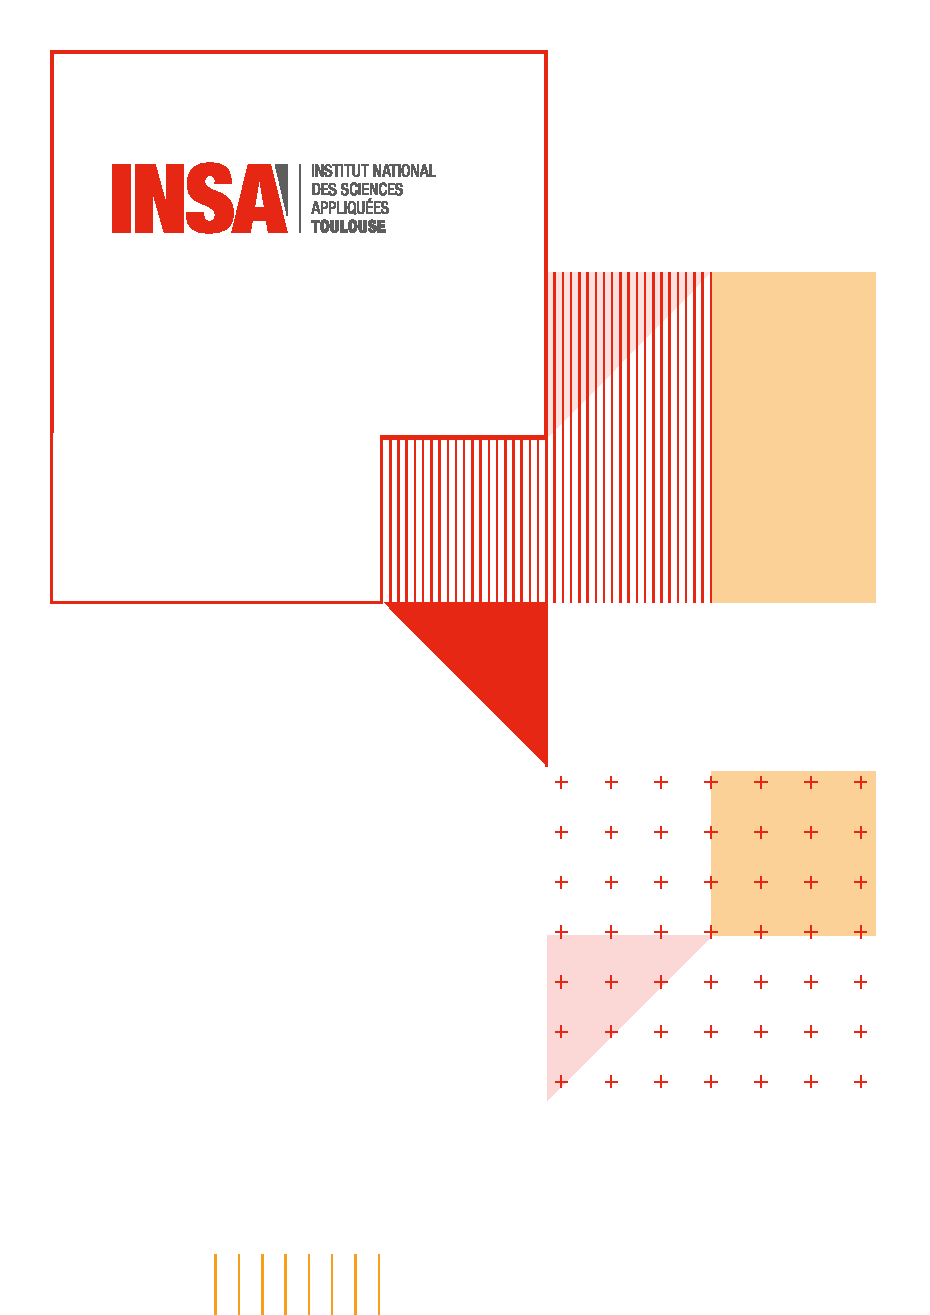
\includegraphics[width=\paperwidth,height=\paperheight]{template/assets/template_first_page.pdf}
    };
    
    \fill[fill=couleurcarre]([xshift=-4.7cm, yshift=-4.5cm]current page.north east) rectangle ++(3.5cm, 3.5cm);
    
    % Ajouter du texte à une position spécifique
    \node at (2.1, -4) {\LARGE \bfseries \MakeUppercase{\sffamily \titre}};
    \node at (6.8, -7) {\large \firstcouverture};
    \node at (6.8, -17) {\secondcouverture};
    %\node at (11.5, -12.2) {\includegraphics[height=3cm]{\imagecouverture}};
    \node at (15.05, -0.3) {\includegraphics[width=3cm]{\imagecouverture}};
\end{tikzpicture}
\newpage
\AddToShipoutPicture{\BackgroundPic}  % ne pas toucher
    \begin{tikzpicture}[remember picture, overlay]
  
    \fill[fill=couleurcarre]([xshift=-4.7cm, yshift=-4.5cm]current page.north east) rectangle ++(3.5cm, 3.5cm);
    
    % Ajouter du texte à une position spécifique
    \node at (2.1, -4) {\LARGE \bfseries \MakeUppercase{\sffamily \titre}};
    \node at (6.8, -7) {\large \firstcouverture};
    \node at (6.8, -17) {{\sffamily\secondcouverture}};
    %\node at (11.5, -12.2) {\includegraphics[height=3cm]{\imagecouverture}};
    \node at (15.05, -0.3) {\includegraphics[width=3cm]{\imagecouverture}};
\end{tikzpicture}
\newpage
    
    % commentez les sections qui ne vous concernent pas
    \psection{Note de confidentialité}
Le présent rapport est classé confidentiel. En conséquence, la divulgation de son contenu à une personne extérieure au corps professoral de l’INSA ou à une personne extérieure à l’entreprise \aremplir{} est interdite.
\newpage
    \psection{Remerciements}
Pour leur aide dans la construction de ce travail, je tiens à remercier plusieurs personnes.\\
Qu’elles trouvent ici l’expression de mes plus sincères remerciements pour leurs précieux conseils.\\\\
Pour cela, je tiens tout d’abord à exprimer ma reconnaissance envers\\
Je remercie tout particulièrement\\
Je remercie aussi spécialement\\

\newpage
    \psection{Abstract}
\aremplir

\newpage
    
    % Table des matières
\tableofcontents
\thispagestyle{empty} % pas de numéro de page sur cette page
\newpage

\pagenumbering{arabic} % Numérotation en chiffres romains (i, ii, iii, ...)
\setcounter{page}{1} % ne pas toucher
    
    % début du contenu
    \psection{Introduction}
Une introduction

\newpage
\section{Section de contenu}
\subsection{sous section}
Ici je cite une grande référence \cite{test}

\section{Une autre section}
\begin{figure}[h]
    \centering
    \includegraphics[width=0.5\textwidth]{example-image} % Remplacez par votre image
    \caption{Ceci est un exemple de figure.}
    \label{fig:example}
\end{figure}

\begin{table}[h]
    \centering
    \caption{Ceci est un exemple de tableau.}
    \begin{tabular}{|c|c|c|}
        \hline
        Colonne 1 & Colonne 2 & Colonne 3 \\ \hline
        Donnée 1  & Donnée 2  & Donnée 3  \\ \hline
        Donnée 4  & Donnée 5  & Donnée 6  \\ \hline
    \end{tabular}
    \label{tab:example}
\end{table}

\section{Another section}
\subsection{Une sous section}
\subsubsection{Une sous sous section}
Un mot compliqué\footnote{Une note de bas de page}

\newpage
\psection{Conclusion}
Une conclusion
    
    % commentez les sections qui ne vous concernent pas
    \newpage
\psection{Bibliographie}
\printbibliography[heading=none]
    \newpage
\psection{Lexique}
\aremplir
    \newpage
\psection{Liste des figures et tableaux}
\listoffigures
\listoftables
\thispagestyle{empty} % pas de numéro de page sur cette page
    
    % annexes
    \newpage
\appendix
\thispagestyle{empty}
\psection{Table des annexes}
\addtocontents{toc}{\protect\setcounter{tocdepth}{0}} % Désactivation de la table des matières

% Personnalisation de la table des annexes
\renewcommand{\stctitle}{}                          % Titre (issue with previous subsection showing up)
\renewcommand\thesubsection{A\arabic{subsection}}   % Numérotation
\renewcommand{\stcSSfont}{}                         % Police normale, pas en gras
\mtcsetrules{secttoc}{off}                          % Désactivation des lignes en haut et en bas de la table

% Affichage de la table des annexes
\secttoc


\newpage
% Annexe 1
\subsection{Annexe A}
Contenu de l'annexe A.

\newpage
% Annexe 2
\subsection{Annexe B}
Contenu de l'annexe B.
    
    \newpage
\AddToShipoutPicture{} 
\thispagestyle{empty} % pas de numéro de page sur cette page
\begin{tikzpicture}[remember picture, overlay]
    \node[anchor=south west, inner sep=0] at (current page.south west) {
        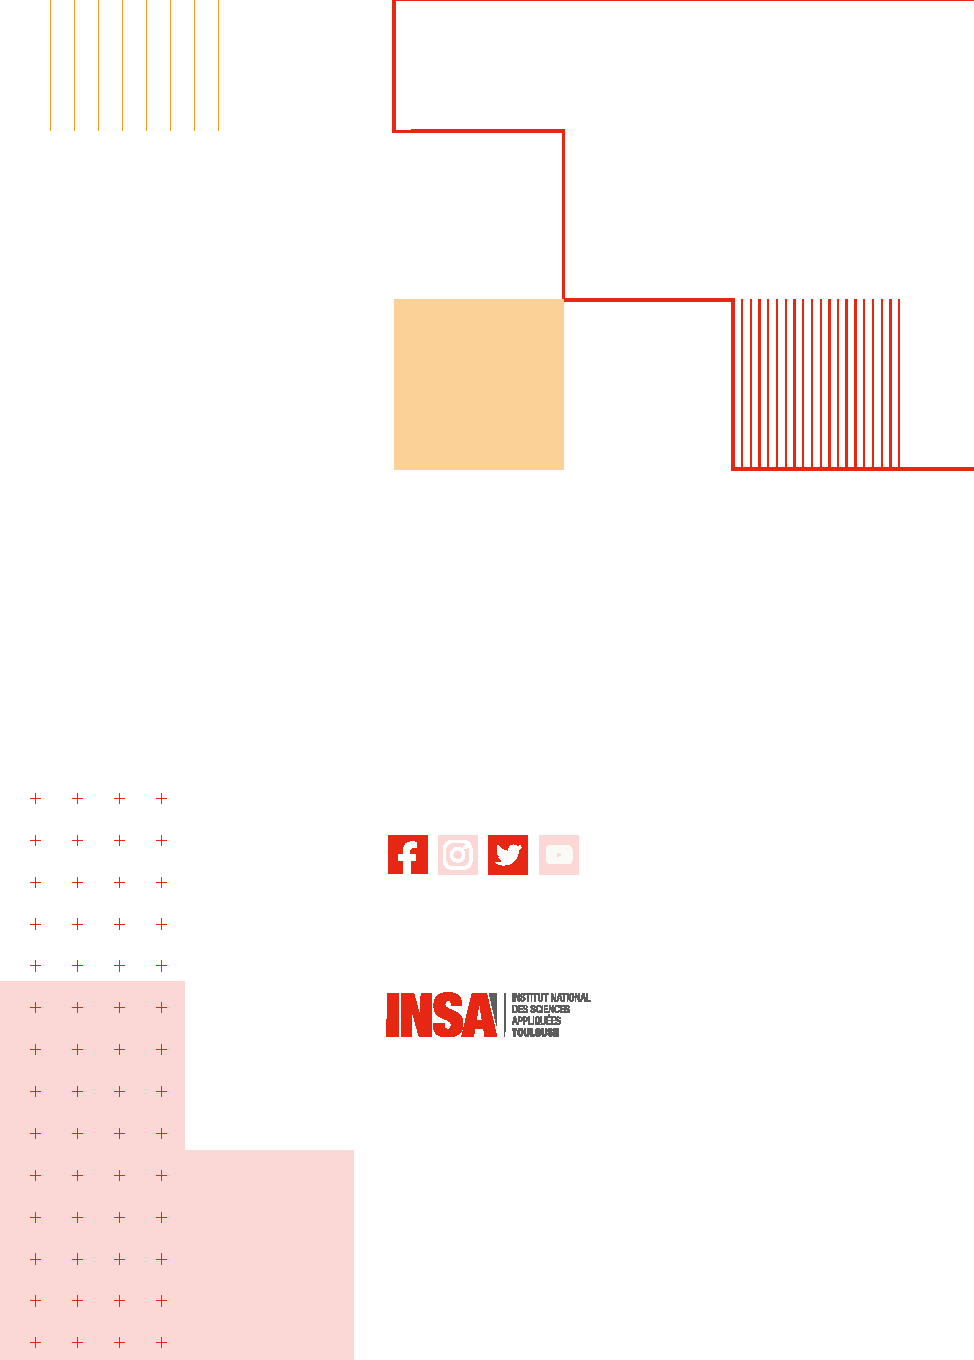
\includegraphics[width=\paperwidth,height=\paperheight]{template/assets/template_last_page.pdf}
    };
    \node at (12.9, -13) {
        \parbox{\textwidth}{
            \large
            \textbf{INSA TOULOUSE}\\
            135 avenue de Rangueil\\
            31400 Toulouse
            \vspace{0.6em}\\
            Tel: +33 (0)5 61 55 95 13\\
           \href{https://www.insa-toulouse.fr/}{\textbf{www.insa-toulouse.fr}}
        }
    };

    % Des logos cliquables
    \node at (5.53, -15.15) {\href{https://www.facebook.com/INSAToulouse/}{
\includegraphics[width=0.8cm]{template/assets/carre.png}}};
    \node at (6.64, -15.15) {\href{https://www.instagram.com/insatoulouse/}{
\includegraphics[width=0.8cm]{template/assets/carre.png}}};
    \node at (7.75, -15.15) {\href{https://x.com/insatoulouse}{
\includegraphics[width=0.8cm]{template/assets/carre.png}}};
    \node at (8.89, -15.15) {\href{https://www.youtube.com/user/insatoulouse}{
\includegraphics[width=0.8cm]{template/assets/carre.png}}};
\end{tikzpicture} % ne pas toucher
\end{document}
